\documentclass[%
    %handout
]{beamer}
\usepackage{graphicx} % For including single page pdfs
\usepackage{bm}       % bold math
\usepackage{pgffor}   % for loop
\usepackage{tikz}
\usetikzlibrary{positioning}

\usepackage{layouts}
\usepackage{hyperref}
\usepackage{cambridge_lecture}

% todo 
% - Ligo actual data
% -define IMRPhenom, EOBNR




\setbeamertemplate{navigation symbols}{} % Turn off that bottom bar


\title{Quantised primordial power spectra}
\subtitle{\tiny PARALLEL SESSION: COSMOLOGY - EARLY UNIVERSE AND THE ORIGIN OF STRUCTURE (F)}
\author[Handley] % (optional, for multiple authors)
{Will Handley\\ \small{wh260@cam.ac.uk}}
\institute[University of Cambridge] % (optional)
{%
Kavli Institute for Cosmology \\
Astrophysics Group \\
Cavendish Laboratory \\
University of Cambridge
}
\date{14:30, Monday 16\textsuperscript{th} December 2019}

\usepackage{calculator}

\newcommand{\cols}[3][0.5]{%
    \SUBTRACT{1.}{#1}{\wdthb}
    \begin{columns}
        \begin{column}{#1\textwidth}
            #2
        \end{column}
        \begin{column}{\wdthb\textwidth}
            #3
        \end{column}
    \end{columns}
}

\newcommand{\figname}{}
\newenvironment{figright}[2][0.5]{%
    \renewcommand{\figname}{#2}
    \SUBTRACT{1.}{#1}{\wdthb}
    \begin{columns}
        \begin{column}{#1\textwidth}
        }{%
        \end{column}
        \begin{column}{\wdthb\textwidth}
            \includegraphics[width=\textwidth]{\figname}
        \end{column}
    \end{columns}
}

\newcommand{\dfigname}{}
\newenvironment{dfigright}[3][0.5]{%
    \renewcommand{\figname}{#2}
    \renewcommand{\dfigname}{#3}
    \SUBTRACT{1.}{#1}{\wdthb}
    \begin{columns}
        \begin{column}{#1\textwidth}
        }{%
        \end{column}
        \begin{column}{\wdthb\textwidth}
            \includegraphics[width=\textwidth]{\figname}
            \includegraphics[width=\textwidth]{\dfigname}
        \end{column}
    \end{columns}
}



\newenvironment{figleft}[2][0.5]{%
    \SUBTRACT{1.}{#1}{\wdthb}
    \begin{columns}
        \begin{column}{#1\textwidth}
            \includegraphics[width=\textwidth]{#2}
        \end{column}
        \begin{column}{\wdthb\textwidth}
        }{%
        \end{column}
    \end{columns}
}

\newenvironment{dfigleft}[3][0.5]{%
    \SUBTRACT{1.}{#1}{\wdthb}
    \begin{columns}
        \begin{column}{#1\textwidth}
            \includegraphics[width=\textwidth]{#2}
            \includegraphics[width=\textwidth]{#3}
        \end{column}
        \begin{column}{\wdthb\textwidth}
        }{%
        \end{column}
    \end{columns}
}


\newcounter{numimages}

\newenvironment{multifig}[1]{%
    \begin{frame}
        \pdfximage{#1}%
        \setcounter{numimages}{\the\pdflastximagepages}
        \addtocounter{numimages}{-1}

        \begin{tikzpicture}[remember picture, overlay]
            \foreach \pagenum in {1,...,\thenumimages} {%
                \node<handout:0|beamer:\pagenum>[anchor=center] at (current page.center) {
                \includegraphics[width=\textwidth,page=\pagenum]{#1}}; 
            }
            \addtocounter{numimages}{1}
            \node<handout:1|beamer:\thenumimages>[anchor=center] at (current page.center) {
            \includegraphics[width=\textwidth,page=\thenumimages]{#1}}; 
        \end{tikzpicture}
    }{%
    \end{frame}
}



\begin{document}

\begin{frame}
  \titlepage
\end{frame}


\begin{frame}
\frametitle{Quantised primordial power spectra}
\tableofcontents
\end{frame}

\section{Observational motivations for quantised primordial power spectra}
\begin{frame}
    \frametitle{Features in the Planck data?}
    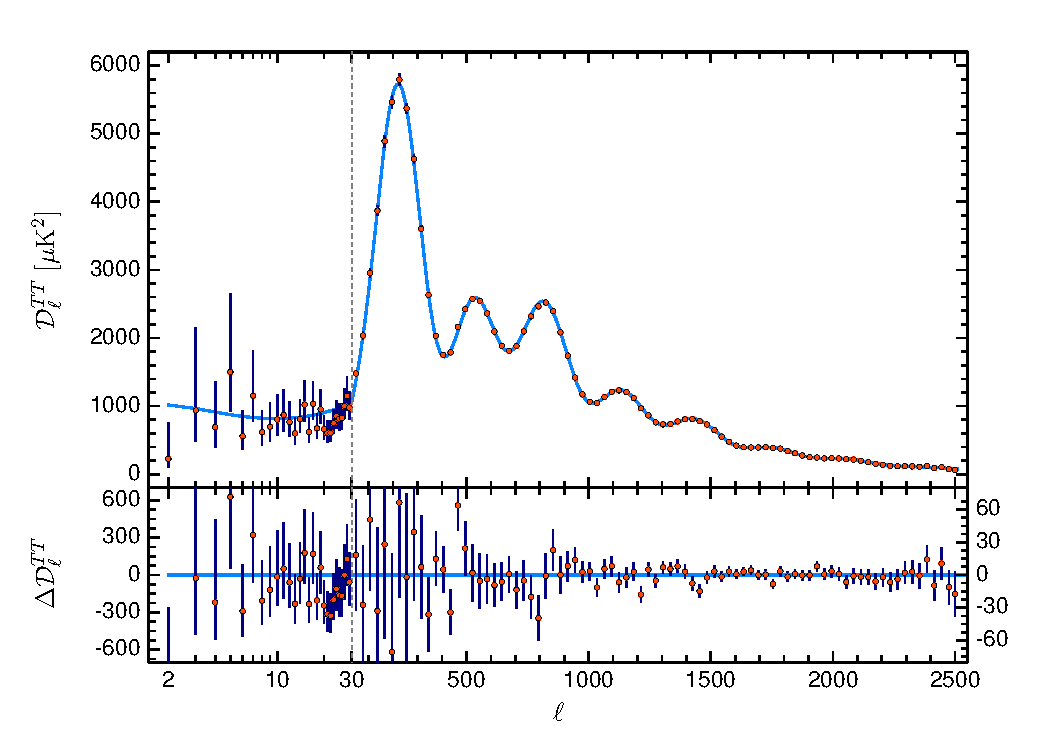
\includegraphics[width=\textwidth]{coadded_TT}
\end{frame}

\begin{frame}
    \frametitle{Features in the Planck data?}
    Normalise residuals to have unit standard deviation:

    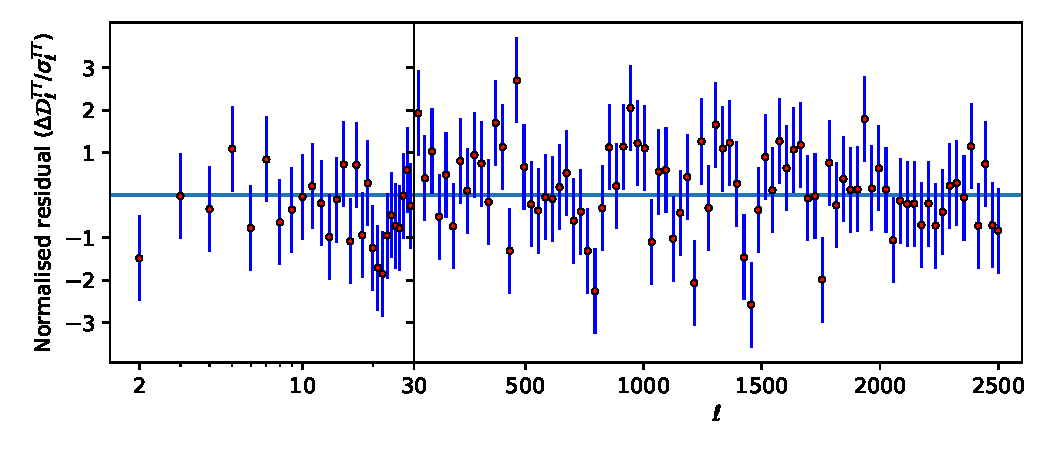
\includegraphics[width=\textwidth]{residuals}

    \begin{enumerate}
        \item low quadrupole ($\ell=2$) and suppression of power $\ell<30$.
        \item $\ell\sim20$ feature.
        \item (faint) oscillatory characteristics in high-$\ell$ residuals.
    \end{enumerate}
\end{frame}

\begin{frame}
    \frametitle{Quantised primordial power spectra}
    \begin{itemize}
        \item From inflation, primordial power spectrum $\mathcal{P}_\mathcal{R}(k)\approx A_s{\left( \frac{k}{k_*} \right)}^{n_s-1}$.
        \item What if, instead of a continuous set of wavevectors, only a discrete set are allowed?
        \item Practically amounts to changing transfer convolution: \[C_\ell \sim \int \mathcal{P}_\mathcal{R}(k) \Delta(k) dk \to \sum\limits_{k_i\in {\text{allowed } k}}\mathcal{P}_\mathcal{R}(k_i) \Delta(k_i)\].
        \item For example, allowed $k$ could have linear spacing $\Delta k$, starting at $k_0$.
        \item Quantisation occurs naturally in closed universes, but mechanisms exist for creating the same in flat or open universes.
        \item ``Improved cosmological fits with quantized primordial power spectra'' (Bartlett, Handley \& Lasenby, Jan 2020).
    \end{itemize}
\end{frame}

\begin{frame}
    \frametitle{Quantised primordial power spectra}
        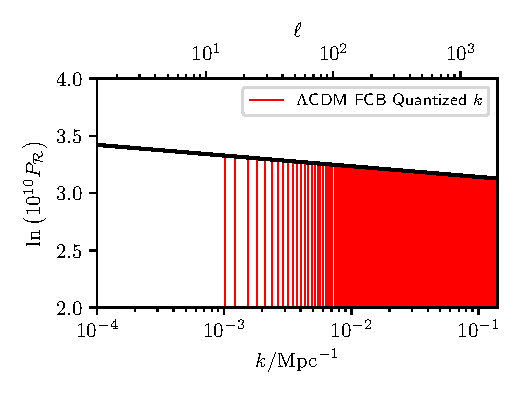
\includegraphics[width=\textwidth]{Quantised_Primordial}
\end{frame}



\begin{frame}
    \frametitle{Physical effects of quantisation}
    \centerline{%
        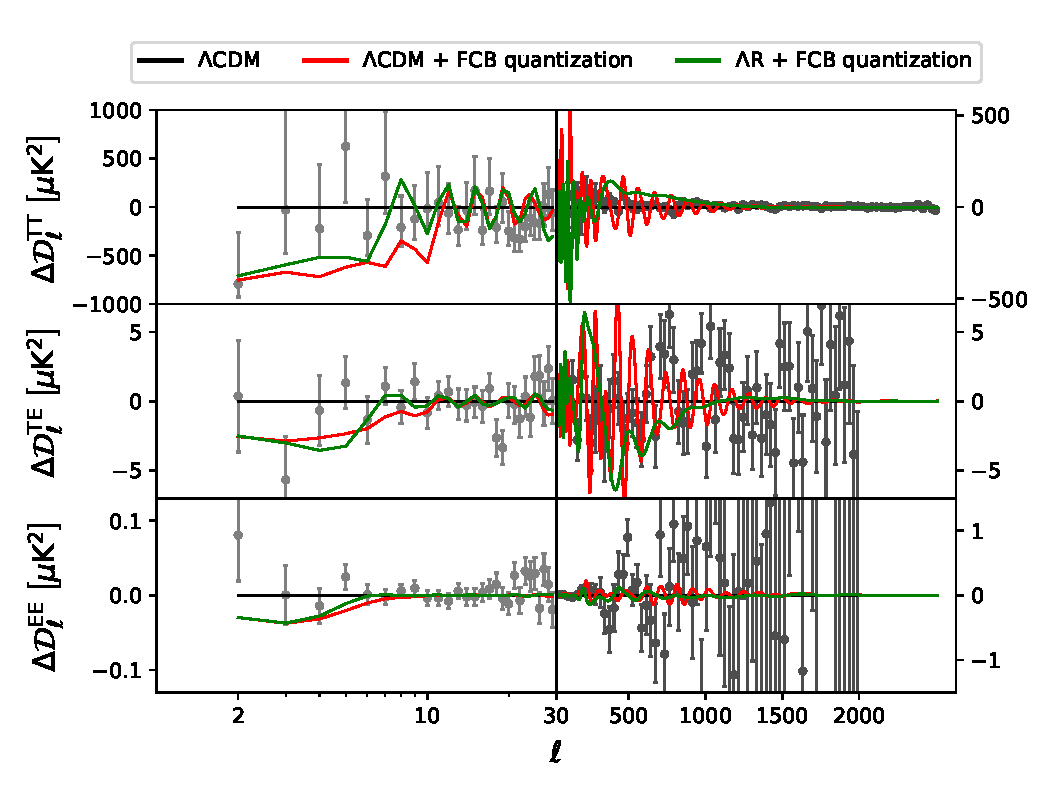
\includegraphics[width=0.95\textwidth]{all_delta_dl_fcb}
    }
\end{frame}

\begin{frame}
    \frametitle{Optimal quantised spectra, $\Delta\chi^2=-8.55$}
    \framesubtitle{Best-fit with Planck 2018 TT,TE,EE+low$\ell$+lowE+lensing likelihood}
    \centerline{%
        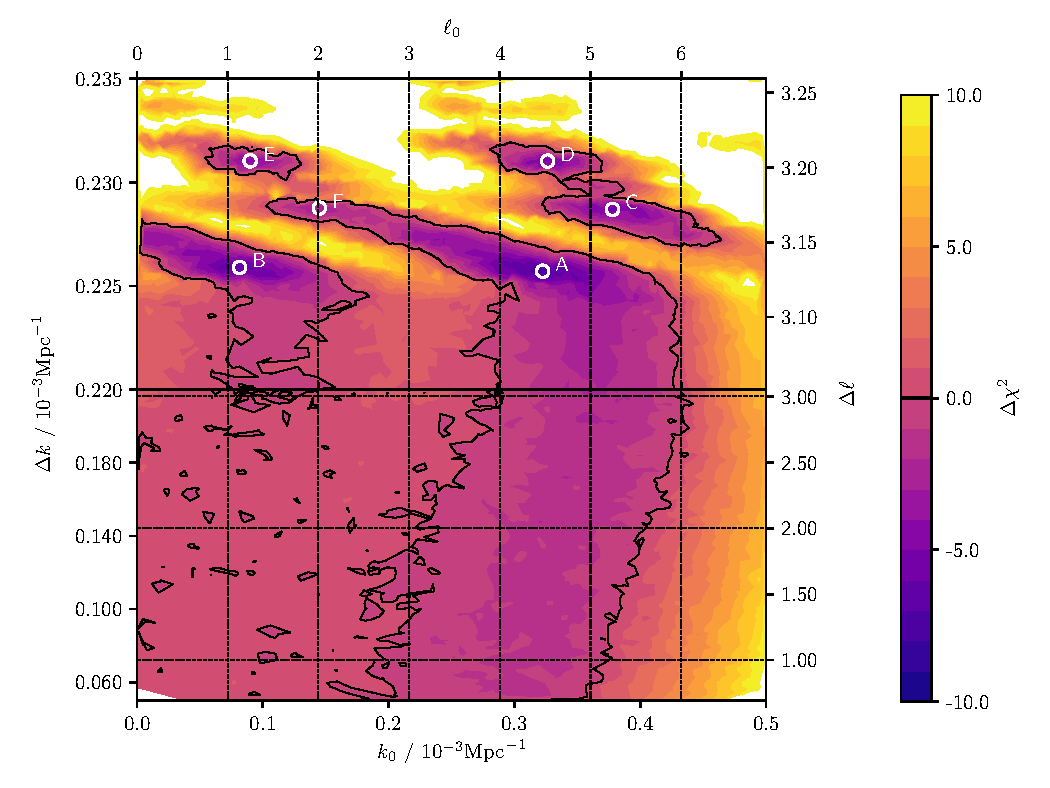
\includegraphics[width=0.9\textwidth]{contour_plot_twoscales}
    }

    Plot of residuals
\end{frame}

\begin{frame}
    \frametitle{Breakdown of fit}
    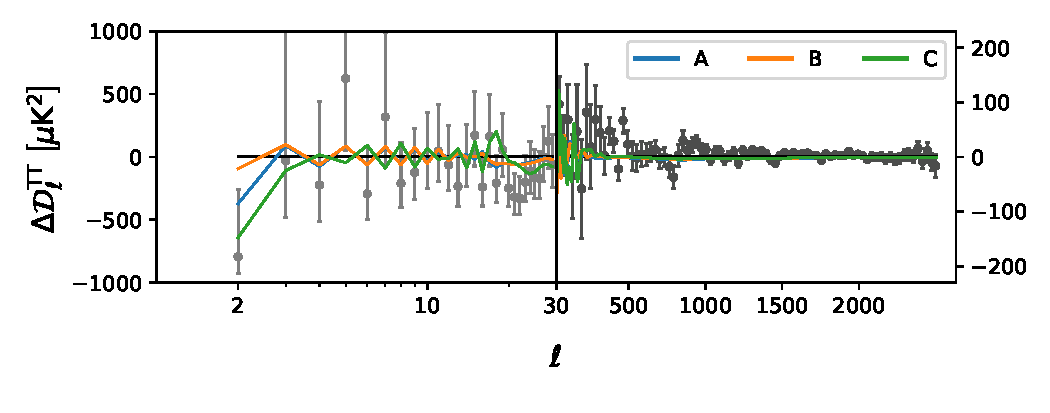
\includegraphics[width=\textwidth]{TT_linear_dl}

    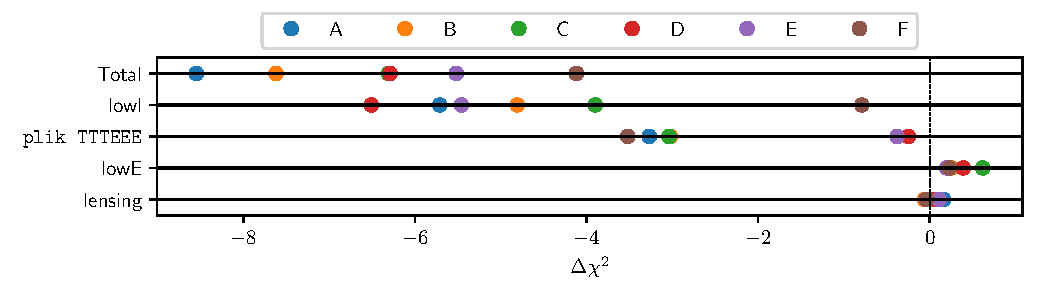
\includegraphics[width=\textwidth]{chi2_contributions}

\end{frame}

\begin{frame}
    \frametitle{How good are these fits?}
    \begin{itemize}
        \item $\Delta\chi^2=-8.55$ is nominally quite an improvement on $\Lambda$CDM.
        \item This comes at the cost of two new parameters associated with the lowest wavenumber $k_0$ and quantisation spacing $\Delta k$.
        \item The parameters are also finely tuned, incurring an Occam penalty in the Bayesian evidence similar in degree to the improved fit.
        \item Ideally would have a models that are more predictive.
    \end{itemize}
    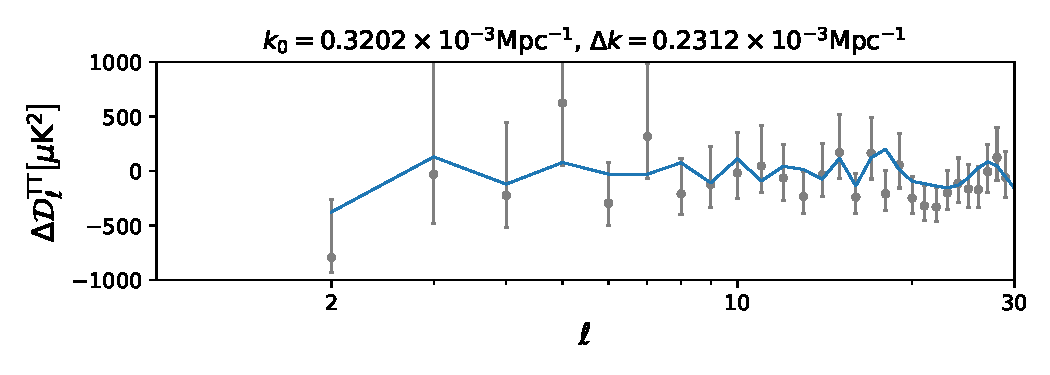
\includegraphics[width=\textwidth]{best_lowl}
\end{frame}

\section{Future conformal boundary theories}

\begin{frame}
    \frametitle{The future conformal boundary}

    \begin{itemize}
        \item Extrapolating our current cosmology, the universe ``ends'' in a Dark energy dominated phase.
        \item As $t\to\infty$, the universe enters a de-Sitter state $a\sim e^{H_\infty t}\to\infty$.
        \item This is a coordinate singularity, at a finite conformal time in the future.
        \item Evolutions of various cosmological components may be continued through this ``future conformal boundary''.
        \item Distinct from Penrose's conformal cyclic cosmologies (CCCs).
        \item ``Radiation, Cold Dark Matter Perturbations and the Future Conformal Boundary'' (Lasenby, Handley et al, Jan 2020).
    \end{itemize}
\end{frame}

\begin{frame}
    \frametitle{Evolution through the future conformal boundary}
    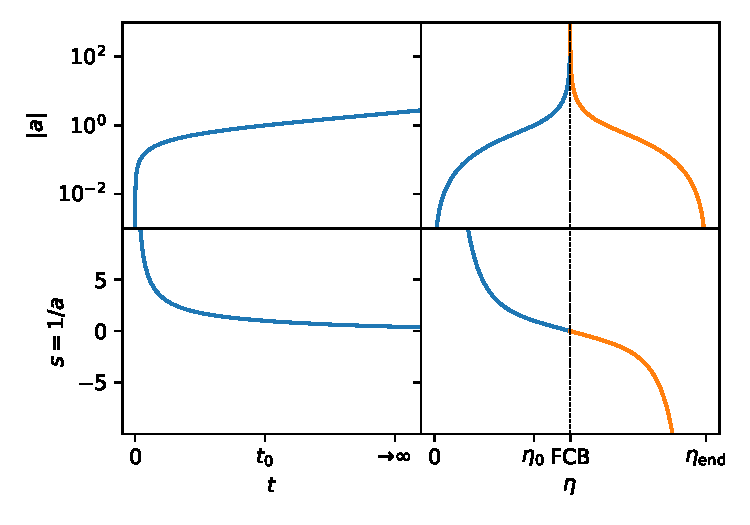
\includegraphics[width=\textwidth]{evolution}
\end{frame}

\begin{frame}
    \frametitle{Consequences of the future conformal boundary}
    Theoretical observations:
    \begin{itemize}
        \item The scale factor $a$ is not a physical quantity.
        \item Metric: $dt^2 - a^2 dx^2 \Rightarrow$  physics is blind to the sign of the scale factor.
        \item $s = 1/a$ would be equally appropriate as a variable.
        \item $s$ remains finite and smooth through the boundary where $a\to\infty$.
    \end{itemize}
    \vspace{10pt}
    Physical consequences:
    \begin{itemize}
        \item For a perturbative approach to be valid, first-order perturbations must remain finite at all times.
        \item Requiring this at the beginning and end of the universe means only a discrete set of wavenumbers are allowed.
    \end{itemize}
\end{frame}

\begin{frame}
    \frametitle{Allowed wavenumbers}
    \centerline{
    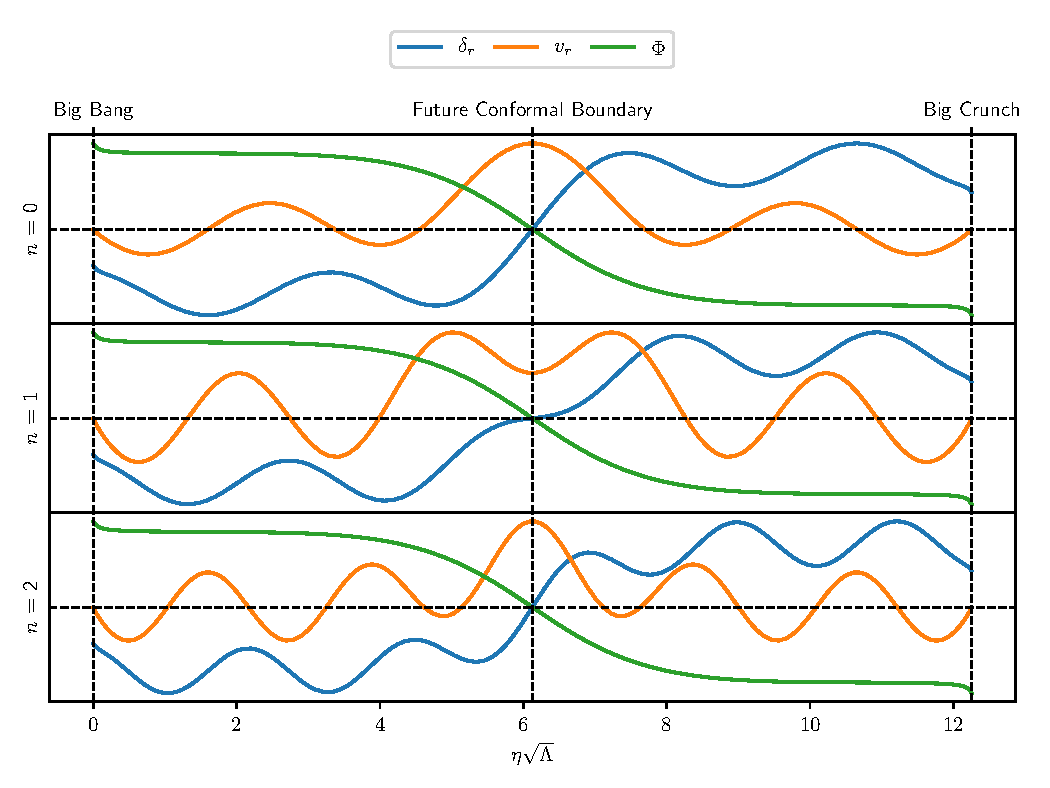
\includegraphics[width=0.95\textwidth]{first_allowed_pert}
    }
\end{frame}

\begin{frame}
    \frametitle{Poor predictions in practice}
    \begin{figright}[0.27]{all_delta_dl_fcb}
        \begin{itemize}
            \item $\Delta k = 0.272 \times 10^{-3}$\\
            \item $k_0=0.701 \times 10^{-3}$
            \item Worse fitting than continuous spectra
        \end{itemize}
    \end{figright}
\end{frame}

\begin{frame}
    \frametitle{The future of future conformal boundary theories}
    Key points:
    \begin{itemize}
        \item The quantisations predicted by future conformal boundary theories are of the correct order of magnitude.
        \item Full analyticity is challenging for matter: Is $\rho_\mathrm{m}\sim a^{-3}\text{ or }|a|^{-3}$?
        \item Correcting this discrepancy may be the key to bringing these theories into observational consistency.
    \end{itemize}
    \vspace{10pt}
    Future work:
    \begin{itemize}
        \item How does inflation fit into this picture?
        \item Can a compensator field $\phi$ create a full analytic continuation?
    \end{itemize}
\end{frame}

\section{Kinetic initial conditions}
\begin{frame}
    \frametitle{Kinetic initial conditions}
    \begin{figright}[0.67]{background}
        \begin{itemize}
            \item If inflation starts late, effects of finite inflation may be observable.
            \item ``Just enough inflation'' theory: $N_\mathrm{tot}\sim N_\star+10$.
            \item Suppression of power and features in spectra.
            \item Pre-inflationary phase generically has $\dot\phi^2\gg V(\phi)$: kinetic dominance.
            \item Solutions and theory independent from $V(\phi)$.
            \item ``Kinetic initial conditions for inflation''\\ (Handley, Hobson \& Lasenby arXiv:1401.2253).
            \item ``A case for kinetically dominated initial conditions for inflation'' (Hergt, Handley, Hobson \& Lasenby arXiv:1809.07185).
        \end{itemize}
    \end{figright}
\end{frame}

\begin{frame}
    \frametitle{Kinetic initial conditions}
    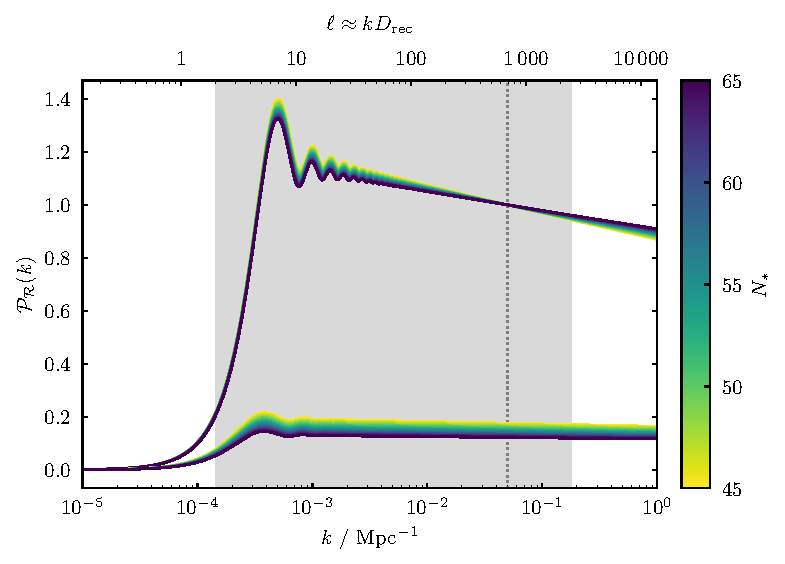
\includegraphics[width=0.49\textwidth]{pps_Nstar}
    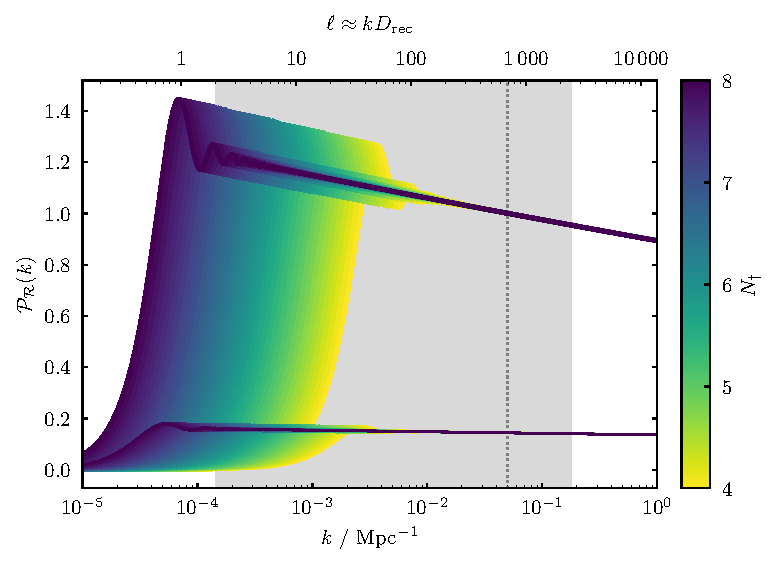
\includegraphics[width=0.49\textwidth]{pps_Ndagg}
    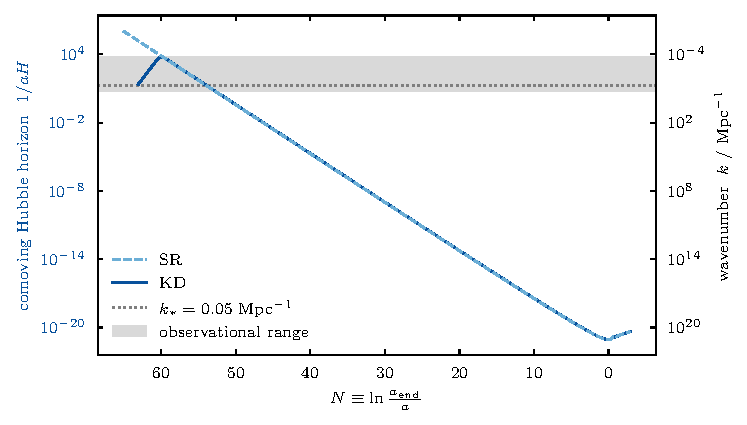
\includegraphics[width=0.49\textwidth]{hubble}
    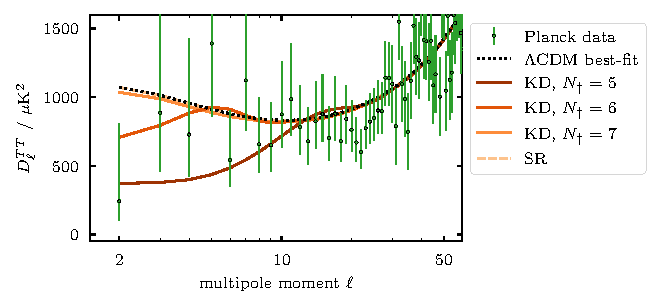
\includegraphics[width=0.49\textwidth]{cmb_KD_Ndagg}
    \begin{itemize}
        \item Hergt, Handley, Hobson \& Lasenby arXiv:1809.07737
    \end{itemize}
\end{frame}

\begin{frame}
    \frametitle{Quantum initial conditions}
    \begin{itemize}
        \item Primordial power spectrum $\mathcal{P}_\mathcal{R}$ governed by freeze-out values of comoving curvature perturbation $\mathcal{R}$.
        \item Traditionally one sets initial conditions for $\mathcal{R}$ (or equivalently the Mukhanov variable $v=z\mathcal{R})$ via quantum mechanical considerations.
        \item For de-Sitter, vacuum clearly defined by Bunch-Davies prescription.
        \item In just enough inflation, for large modes (small $k$) the quantum mechanics is much less clear.
        \item ``Novel quantum initial conditions for inflation''\\
            (Handley, Lasenby \& Hobson arXiv:1607.04148).
    \end{itemize}
\end{frame}

\begin{frame}
    \frametitle{Frozen initial conditions}

    \begin{figright}[0.3]{Exit}
        \begin{itemize}
            \item Proposal: 
                \begin{align}
                    \lim\limits_{t\to 0}&\:|\mathcal{R}|\sim\mathrm{const} \nonumber\\
                    \lim\limits_{t\to 0}&\:\dot{\mathcal{R}}=0 \nonumber
                \end{align}
            \item Perturbations remain valid.
            \item Cosine mode/real component is selected.
            \item Acoustic oscillations on horizon exit.
        \end{itemize}
    \end{figright}
\end{frame}

\begin{frame}
    \frametitle{Frozen power spectra}
    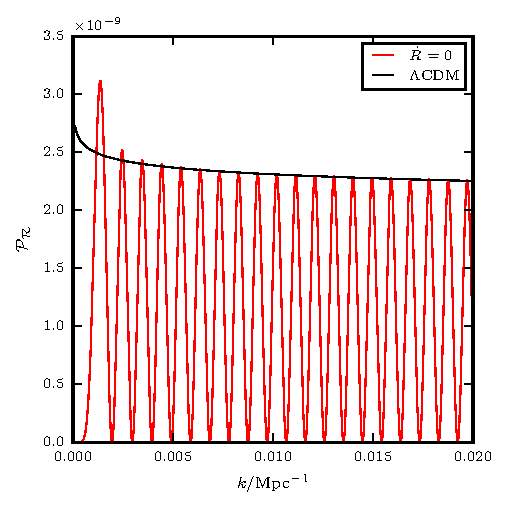
\includegraphics[width=0.49\textwidth]{quantised_pps}
    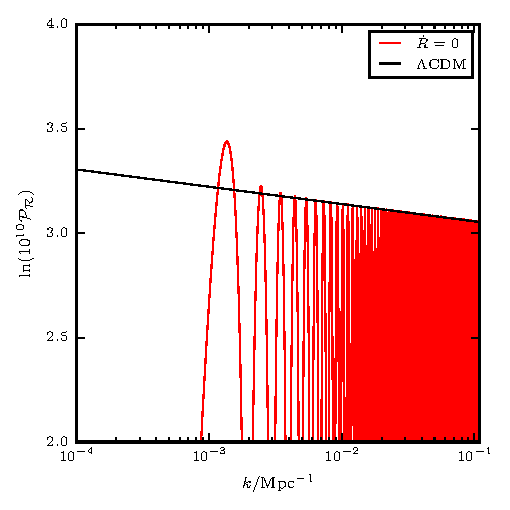
\includegraphics[width=0.49\textwidth]{quantised_pps_log}
    \begin{itemize}
        \item Pseudo quantised power spectrum $\mathcal{P}_\mathcal{R}\approx A_s{\left( \frac{k}{k_*} \right)}^{n_s-1}\times \cos^2(\omega k+\phi)$.
        \item $k_0$, $\Delta k$ are a function of when inflation starts.
        \item ``Rapid numerical solutions for the Mukhanov-Sazaki equation''\\(Haddadin \& Handley, arXiv:1809.11095v2 Jan 2020).
    \end{itemize}

\end{frame}

\begin{frame}
    \frametitle{Observational consequences}
    \centerline{%
        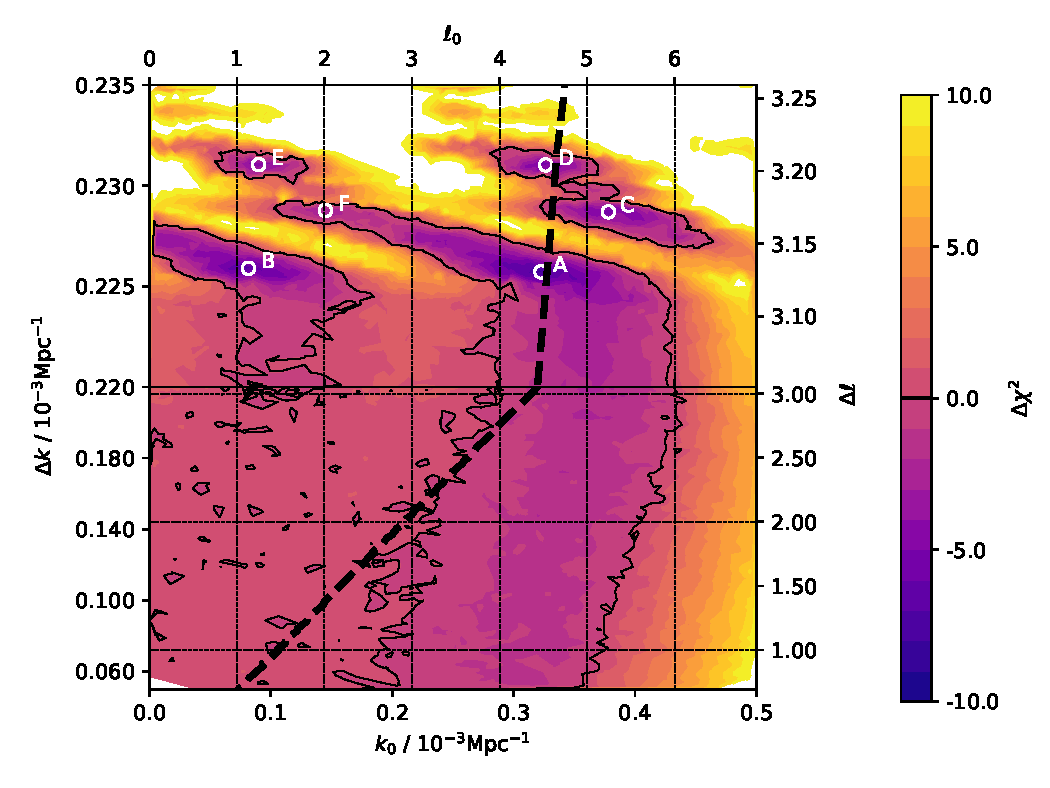
\includegraphics[width=0.95\textwidth]{haddadin}
    }
\end{frame}

\begin{frame}
    \frametitle{Further work}
    \begin{itemize}
        \item Full Bayesian parameter estimation and model comparison.
        \item Quantum consequences/interpretation of frozen initial conditions.
        \item Implications for the effects of the future conformal boundary?
        \item Currently being explored by Thomas Gessey-Jones (Part III student).
    \end{itemize}
\end{frame}

\begin{frame}
    \frametitle{Summary}
    \begin{itemize}
        \item Quantised primordial power spectra have an intriguing observational motivation, able to simultaneously reproduce suppression of low-$\ell$ power, the $\ell\sim20$ feature and oscillations at high $\ell$.
        \item The future conformal boundary is a coordinate singularity, and naturally induces a quantised primordial power spectrum of the correct order of magnitude, but inconsistent with observations.
        \item Kinetic initial conditions/just enough inflation models combined with frozen initial conditions produce a pseudo-quantised spectrum which compellingly can recover the 'sweet spot' best-fit with a single additional cosmological parameter.
    \end{itemize}
\end{frame}

%\begin{frame}
%    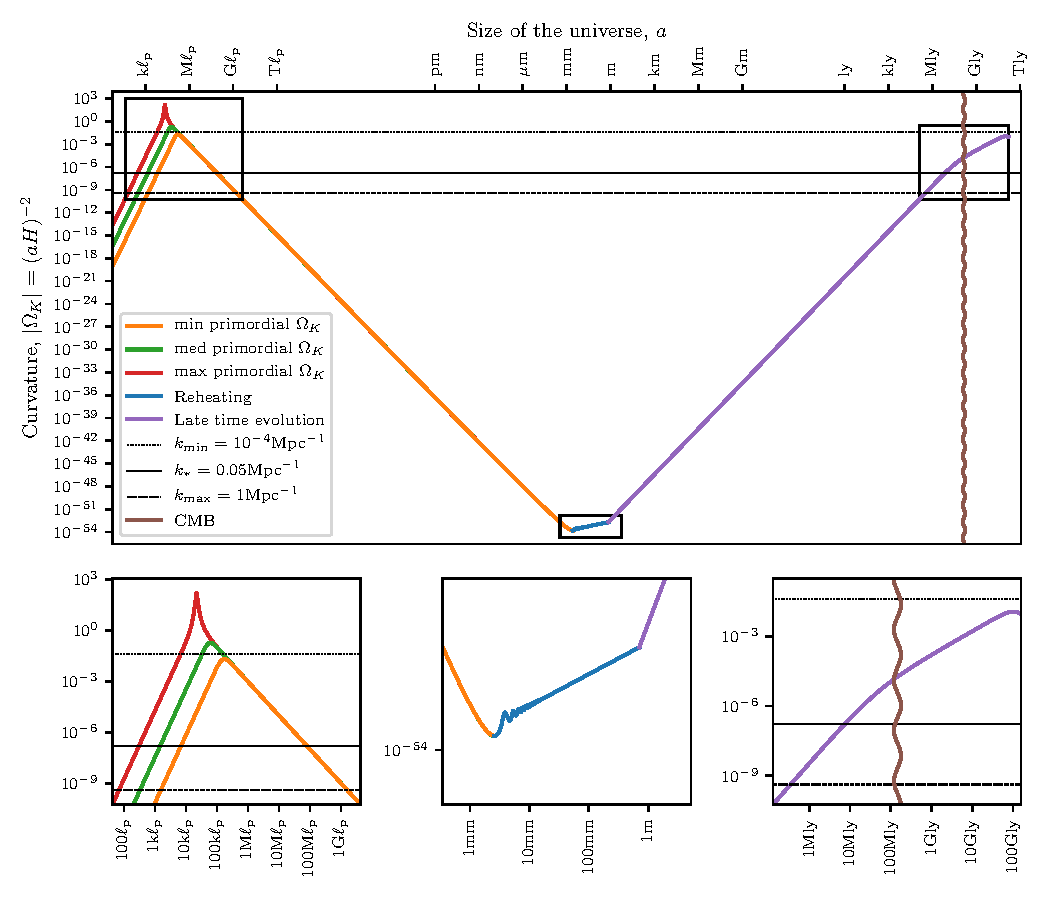
\includegraphics[width=0.8\textwidth]{phi4o3}
%
%    primordial curvature as alternative motivation for just enough inflation
%
%    + other slides
%\end{frame}
%
%\begin{frame}
%    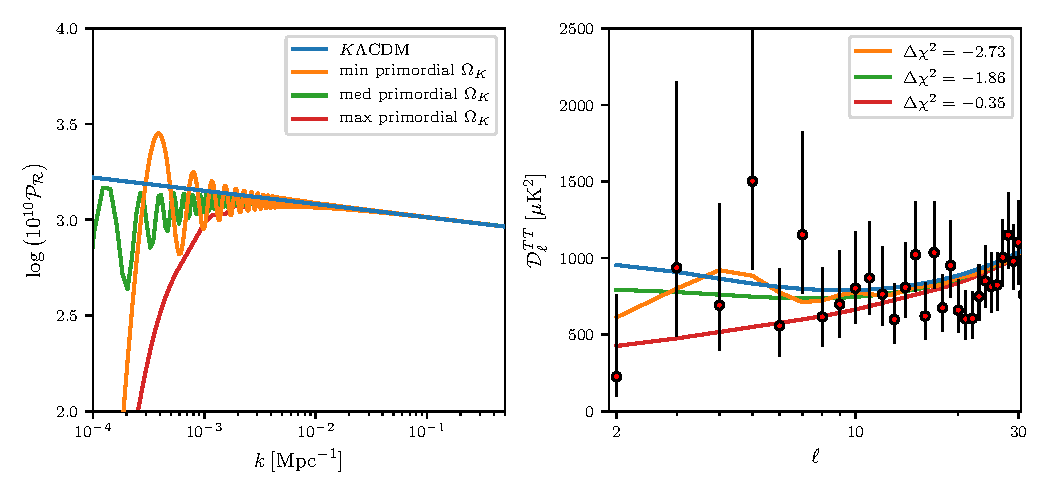
\includegraphics[width=\textwidth]{RST}
%
%    \begin{itemize}
%        \item ``Primordial power spectra for curved inflating universes''\\ Handley arXiv:1907.08524 
%    \end{itemize}
%\end{frame}

\end{document}
